% !TeX spellcheck = en_US
\section{Analysis of Results}\label{sec:results}

After collecting all the data of the Architectural and Test smells we analyzed them. This section discusses the obtained results with the goal of answering the two formulated questions. In particular, we will present the findings for Q1 in Section 3.1 and Q2 in Section 3.2 to facilitate discussion of the results and avoid redundancies.

\subsection{Q1: Correlated increase of Architectural and Test smells}
For every project that we mined and gathered data we compared this data and created a pair of plots, in particular:
\begin{itemize}
  \item The first represents the number of Architectural Smells for the entire project.
  \item The second represents the number of Test Smells for the entire project.
\end{itemize}
The goal of this phase was to observe visually that with an increase of the number of Architectural Smells for the project there was an increase of Test Smells too.

In the images below you can see this parallel increment between the two plots of the same project.

\begin{figure}[htp]
    \centering
    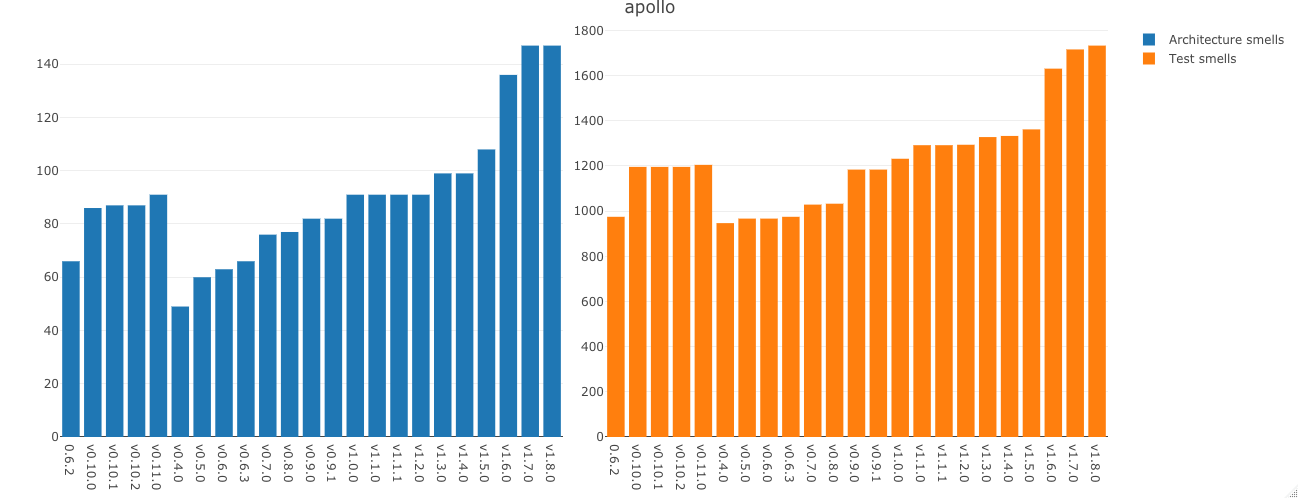
\includegraphics[width=8cm]{img/apollo.png}
    \caption{Project: Apollo}
    \label{fig:apollo}
\end{figure}
\begin{figure}[htp]
    \centering
    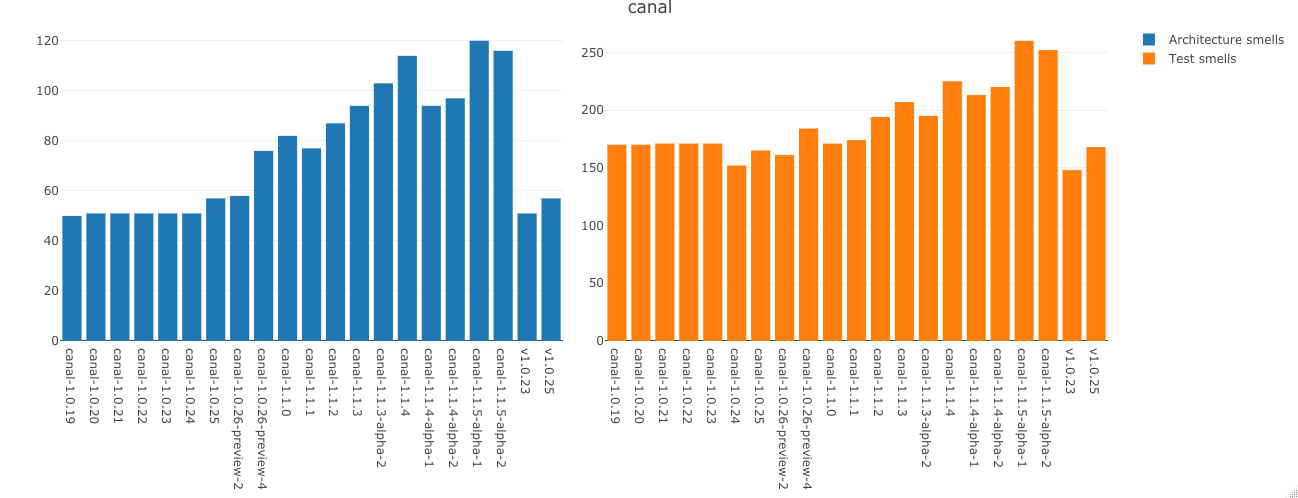
\includegraphics[width=8cm]{img/canal.png}
    \caption{Project: Canal}
    \label{fig:canal}
\end{figure}
\begin{figure}[htp]
    \centering
    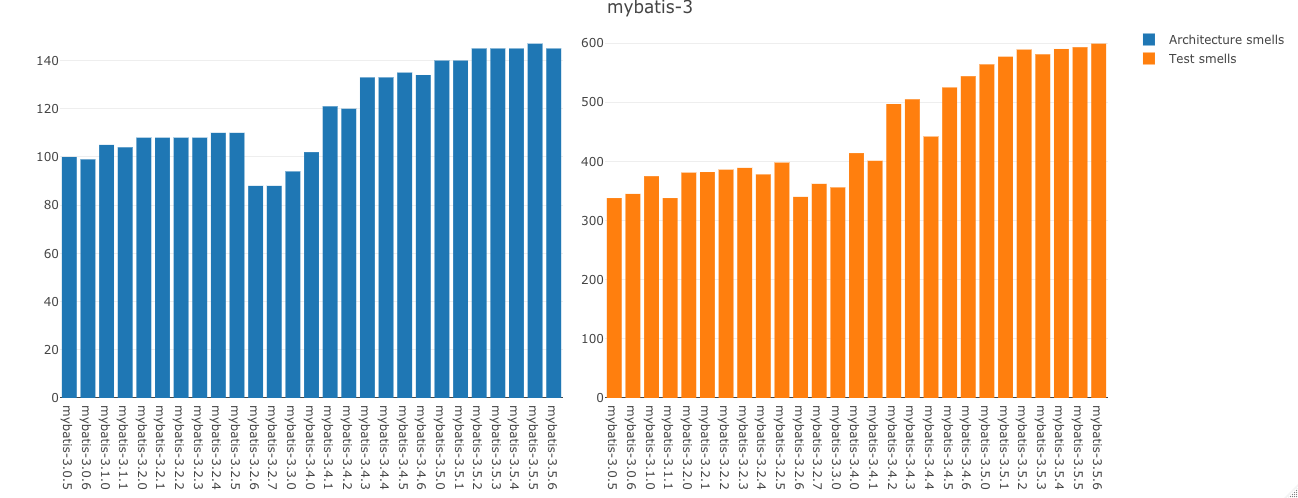
\includegraphics[width=8cm]{img/mybatis-3.png}
    \caption{Project: Mybatis-3}
    \label{fig:mybatis-3}
\end{figure}

For reason of space we reported only a few of the plots of the projects analyzed, but all the other plots are available on the Github repository \cite{IEEEhowto:plotsR}. \par\hfill

As you can observe from the previous plots when there is an increase of Architectural smells (blue plots) there is an increase of Test smells (orange plots) too, and it is also interesting to observe that when the Architectural smells decrease there is a decrease of the Test smells too.\par\hfill

These plots are related to the versions of the projects, so every bar of these represent the number of smells contained in the relative version, while the Architectural smells considered are package-level.\par\hfill

Once computed these, we decided to compute the co-occurrence of the smells\footnote{The counting of paired data within a collection.}, in particular we calculated all the co-occurrence between:
\begin{itemize}
  \item \textit{Architectural Smells - Architectural Smells};
  \item \textit{Test Smells - Test Smells};
  \item \textit{Architectural Smells - Test Smells};
\end{itemize}
As you can see in the Table \ref{co-occurrencesAS} the Architectural Smells considered are at the class level because we compared them with Test Smells that are at a class level too.
In the Table \ref{co-occurrencesTS} there are the co-occurrence of Test Smells, and in the table \ref{co-occurrencesAS-TS} there are the co-occurrence between the Architectural Smells and Test Smells at class level.
The tables in the examples refers to the specific project \textit{"Apollo"} \cite{IEEEhowto:apollo}. 
In the GitHub repository are available the Python scripts to compute it and the result of the computation for all the projects \cite{IEEEhowto:co-occurrence}.

\begin{table}[!ht]
\centering
\caption{Co-occurrences Architectural Smell - Architectural Smell in \emph{Apollo} project.}\label{co-occurrencesAS}
\resizebox{0.5\textwidth}{!}{%
\begin{tabular}{cccccc}
 \csvreader[
  tabular=|r|*{12}{c}|,
  nohead,column count=13,
  table head=\hline,
  late after first line=\\\hline,
  table foot=\hline]{table/apolloArch.csv}%
{}%
{\csviffirstrow{%
  \csvcoli & \myrot{ii} & \myrot{iii} & \myrot{iv} & \myrot{v} & \myrot{vi} & \myrot{vii}
  & \myrot{viii} & \myrot{ix} & \myrot{x} & \myrot{xi} & \myrot{xii} & \myrot{xiii}
}{\csvlinetotablerow}}
\end{tabular}
}
\end{table}

\begin{table}[!ht]
\caption{Co-occurrences Test Smell - Test Smell in \emph{Apollo} project.}\label{co-occurrencesTS}
\resizebox{0.5\textwidth}{!}{%
\begin{tabular}{cccccc}
\csvreader[
  tabular=|r|*{7}{c}|,
  nohead,column count=8,
  table head=\hline,
  late after first line=\\\hline,
  table foot=\hline]{table/apolloTest.csv}%
{}%
{\csviffirstrow{%
  \csvcoli & \myrot{ii} & \myrot{iii} & \myrot{iv} & \myrot{v} & \myrot{vi} & \myrot{vii}
  & \myrot{viii}
}{\csvlinetotablerow}}
\end{tabular}
}
\end{table}

\begin{table}[!ht]
\caption{Co-occurrences Architectural Smell - Test Smell in \emph{Apollo} project.}\label{co-occurrencesAS-TS}
\resizebox{0.5\textwidth}{!}{%
\begin{tabular}{cccccc}
\csvreader[
  tabular=|r|*{7}{c}|,
  nohead,column count=8,
  table head=\hline,
  late after first line=\\\hline,
  table foot=\hline]{table/apolloArchTest.csv}%
{}%
{\csviffirstrow{%
  \csvcoli & \myrot{ii} & \myrot{iii} & \myrot{iv} & \myrot{v} & \myrot{vi} & \myrot{vii}
  & \myrot{viii}
}{\csvlinetotablerow}}
\end{tabular}
}
\end{table}\mbox{}



The Table \ref{co-occurrencesAS} shows clearly that there is the 96\% of probability to find both \emph{Unnecessary Abstraction} and \emph{Unutilized Abstraction}, for example. According to test smells, the table \ref{co-occurrencesTS} shows that there is the 93\% of probability to find \emph{ar1} and \emph{et1} together. Finally, in the table \ref{co-occurrencesAS-TS}, you can see that when there is the smell \emph{Wide Hierarchy} with the 79\% of probability there will be a test smell \emph{ar1}.
\par\hfill

\subsection{Q2: Find association between smells through Association rule}
After that, our goal was to find an association between different objects in a set, find frequent patterns in any information repository. In particular, our purpose was to generate a set of rules called Association Rules, in form \textbf{if this then that}.

Also in this case we considered the three combination of (i) \textit{Architectural Smells - Architectural Smells}, (ii) \textit{Test Smells - Test Smells}, (iii) \textit{Architectural Smells - Test Smells}, where for Architectural Smells we refer to class level.
What we have done here was to create a unique dataset witch contains all the Architectural Smells for all the projects and a unique dataset that contains all the Test Smells for all the projects. After that, we did the inner join between them on the attribute className (in fact for this reason we considered Architectural Smells at class level). The result of this operation was a big dataset that contains for each class several rows with all the smells for all the versions of all the projects. For simplicity in reading, we had added an additional column that contained the smells of that row separated by commas.

Before applying Association Rule mining, we needed to convert data frame into transaction data so that all smells that appeared together in one class were put in one row.
The smells were grouped using NameClass. We did this in R with:

\begin{lstlisting}[language=R]
library(plyr)

transactionData <- ddply(df_join,c("ClassName"),
          function(df_join)paste(df_join$Smells,
                                collapse = ","))
\end{lstlisting}

These data then were saved in a CSV file and then was loaded into an object of the transaction class. This was done by using the R function \verb|read.transactions| with the basket format and converted it into an object of the transaction class. 
With the summary of the transactions we obtained:


\begin{figure}[htp]
    \centering
    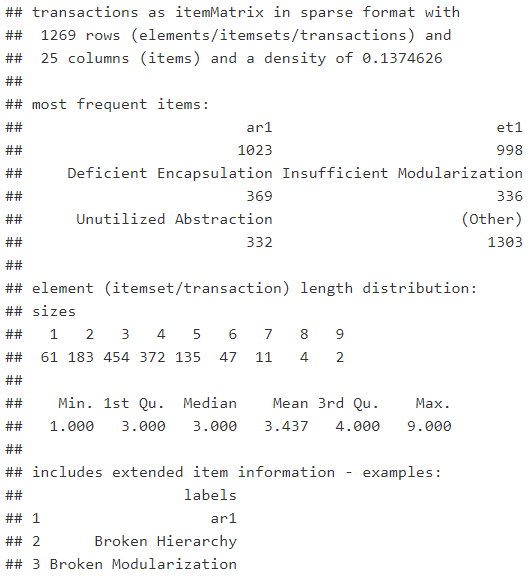
\includegraphics[width=8.5cm]{img/summaryTransaction.PNG}
    \caption{Summary of transaction results}
    \label{fig:summaryTransaction}
\end{figure}

In particular:
\begin{itemize}
  \item There are 1269 transactions (rows) and 25 items (columns). Note that 25 are the smells involved in the dataset and 1269 transactions are collections of these items.
  \item Density tells the percentage of non-zero cells in a sparse matrix. You can say it as the total number of smells that are detected divided by a possible number of smells in that matrix. You can calculate how many items were purchased by using density: $1269 * 25 * 0.1374626 = 4361.0$.
\end{itemize}

Then we computed the item frequency plots for both absolute and relative because if absolute it will plot numeric frequencies of each item independently, if relative it will plot how many times these items have appeared as compared to others. 
\begin{figure}[htp]
    \centering
    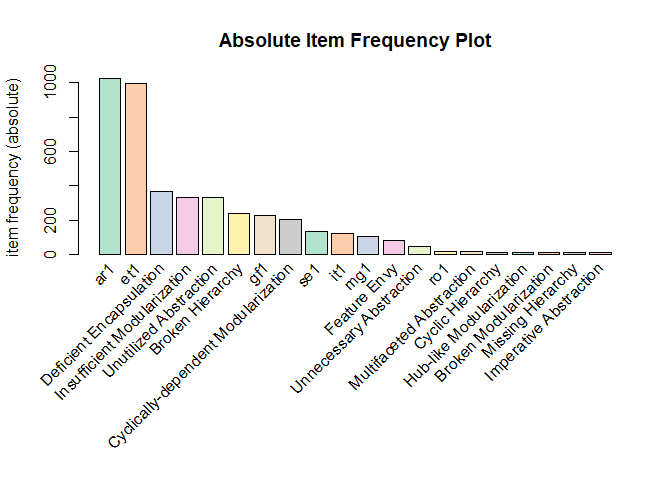
\includegraphics[width=8.5cm]{img/absoluteItemFreq.png}
    \caption{Absolute Item Frequency Plot}
    \label{fig:absoluteItemFreq}
\end{figure}
\begin{figure}[htp]
    \centering
    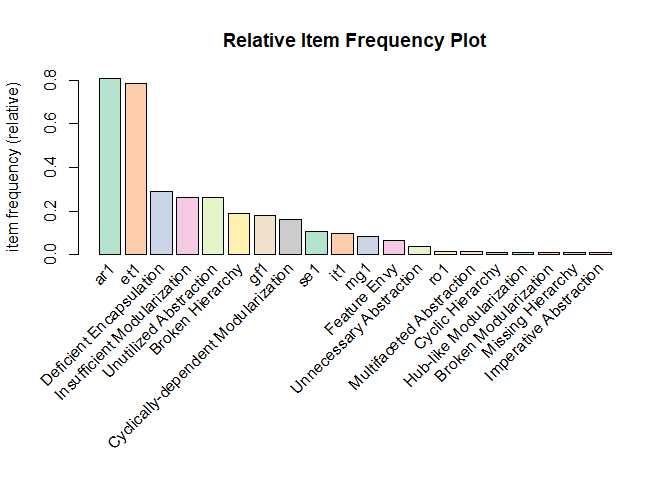
\includegraphics[width=8.5cm]{img/relativeItemFreq.png}
    \caption{Relative Item Frequency Plot}
    \label{fig:relativeItemFreq}
\end{figure}

The next step was to mine the rules using the \textbf{APRIORI} algorithm. We used the function \verb|apriori()| from package \verb|arules|. The apriori takes the transaction data as the transaction object on which mining is to be applied. The parameter that we used for the support was 0.001, and for the confidence was 0.8 (because several works have chosen these thresholds  like \cite{IEEEhowto:associationRules}), then we specified a maximum of 2 items (maxlen), minimum of 2 items (minlen). With the appearance, we specified the LHS (IF part) with the array of Architectural Smells and RHS (THEN part) with the Test Smells.

\begin{lstlisting}[language=R]
design_smells = c('Deficient Encapsulation', 'Unutilized Abstraction', 'Feature Envy',  'Broken Hierarchy', 'Broken Modularization', 'Insufficient Modularization', 'Wide Hierarchy', 'Unnecessary Abstraction', 'Multifaceted Abstraction', 'Cyclically-dependent Modularization','Cyclic Hierarchy', 'Rebellious Hierarchy')

test_smells = c("ar1", "et1", "it1",  "gf1", "se1", "mg1", "ro1")

association.rules <- 
apriori(tr, parameter = list(supp=0.001,                          conf=0.8, minlen=2, maxlen=2),
    appearance = list(lhs=design_smells, rhs=test_smells))
\end{lstlisting}

From this computation with these parameters we obtained 9 rules.


\begin{figure}[htp]
    \centering
    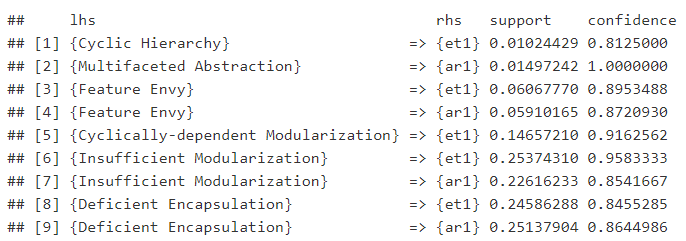
\includegraphics[width=8.5cm]{img/ruleArchTest.PNG}
    \caption{Rule Architectural Smells - Test Smells}
    \label{fig:ruleArchTest}
\end{figure}

Using the above output, you can make analyses such as:
\begin{itemize}
  \item Classes which have design smell \textit{‘Cyclic Hierarchy’} will have the test smell \textit{‘et1’} with support of 0.01 and confidence of 0.81.
  \item Classes which have design smell \textit{‘Multifaceted Abstraction’} will have the test smell \textit{‘ar1’} with support of 0.0149 and confidence of 1.
  \item Classes which have design smell \textit{‘Feature Envy’} will have the test smell \textit{‘et1’} with support of 0.06 and confidence of 0.89.
  \item Classes which have design smell \textit{‘Feature Envy’} will have the test smell \textit{‘ar1’} with support of 0.059 and confidence of 0.87.
\end{itemize}

We did the same thing with both LHS (left part) and RHS (right part) imposed with Architectural Smells, but here we setted the parameter maxlen of the apriori function equals to 4 because with maxlen=2 or maxlen=3 there were less then 2 rules. From this computation we obtained the following 7 rules: \par
\begin{figure}[htp]
    \centering
    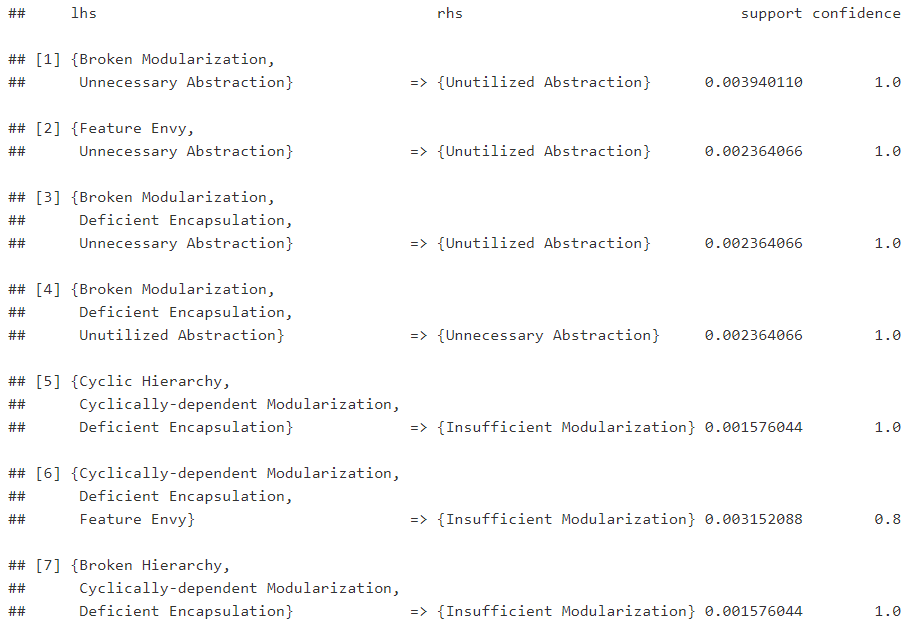
\includegraphics[width=8.5cm]{img/ruleArch.PNG}
    \caption{Rule Architectural Smells - Architectural Smells}
    \label{fig:ruleArch}
\end{figure}
Using the above output, you can make analyses such as:
\begin{itemize}
  \item Classes which have design smells \textit{‘Broken Modularization’} and \textit{‘Unnecessary Abstraction’} will have the design smell \textit{‘Unutilized Abstraction’} with support of 0.0039 and confidence of 1.
  \item Classes which have design smell \textit{‘Feature Envy’} and ‘Unnecessary Abstraction’ will have the design smell \textit{‘Unutilized Abstraction’} with support of 0.0023 and confidence of 1.
\end{itemize}

Finally, we did the same computation to Test Smells to and we called the apriori function with both LHS (left part) and RHS (right part) imposed with Test Smells but here we imposed the maxlen and minlen both equals to 2. From this computation, we obtained 13 rules and we filtered the first 10:
\begin{figure}[htp]
    \centering
    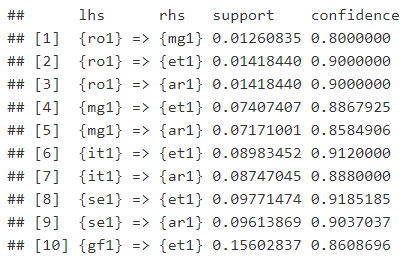
\includegraphics[width=8.5cm]{img/ruleTest.PNG}
    \caption{Rule Test Smells - Test Smells}
    \label{fig:ruleTest}
\end{figure}

Using the above output, you can make analyses such as:
\begin{itemize}
  \item Classes which have test smell \textit{‘ro1’} will have the test smell \textit{‘mg1’} with support of 0.0126 and confidence of 0.8.
  \item Classes which have test smell \textit{‘ro1’} will have the test smell \textit{‘et1’} with support of 0.0141 and confidence of 0.9.
\end{itemize}
\par\hfill

\subsubsection{Visualize Association Rules}

Since there will be hundreds or thousands of rules generated based on data, there are a couple of ways to visualize these association rules.
%\begin{figure}[ht]
%    \centering
%    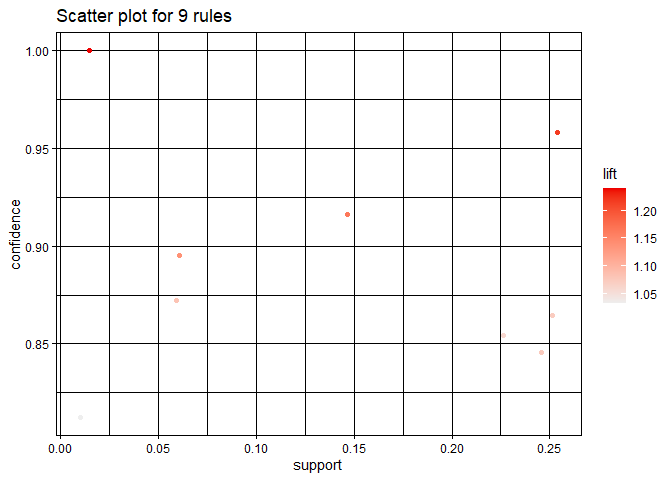
\includegraphics[width=5cm]{img/scatterPlotArchTest.png}
%    \caption{Scatter-Plot Architectural Smells-Test Smell}
%    \label{fig:scatterPlotArchTest}
%\end{figure}
%\begin{figure}[ht]
%    \centering
%    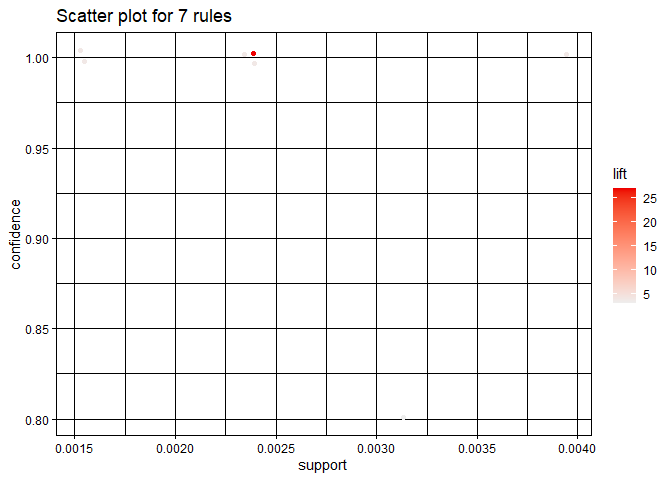
\includegraphics[width=5cm]{img/scatterPlotArch.png}
%    \caption{Scatter-Plot Architectural Smells}
%    \label{fig:scatterPlotArch}
%\end{figure}
%\begin{figure}[ht]
%    \centering
%    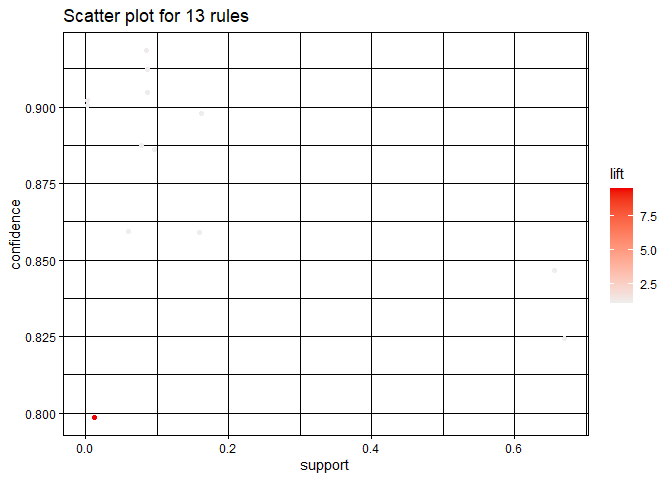
\includegraphics[width=5cm]{img/scatterPlotTest.png}
%    \caption{Scatter-Plot Test Smells}
%    \label{fig:scatterPlotTest}
%\end{figure}

One of the visualization that we computed is the Individual Rule Representation, this representation is also called as Parallel Coordinates Plot.
\begin{figure}[!ht]
    \centering
    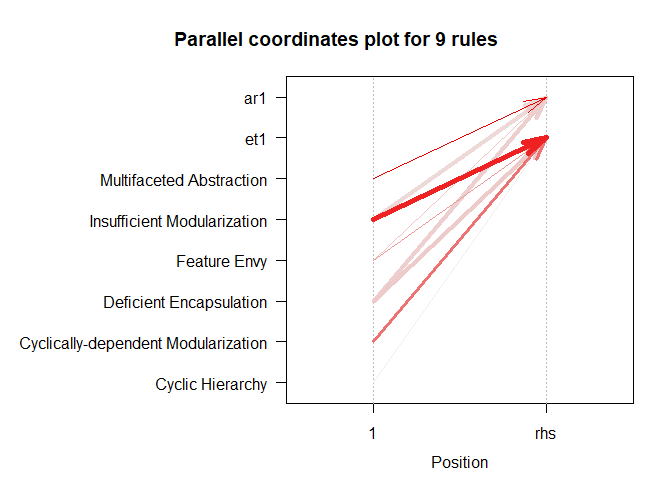
\includegraphics[width=5cm]{img/parallelCoordinateArchTest.png}
    \caption{Parallel Coordinate Architectural Smells-Test Smell}
    \label{fig:parallelCoordinateArchTest}
\end{figure}
\begin{figure}[!ht]
    \centering
    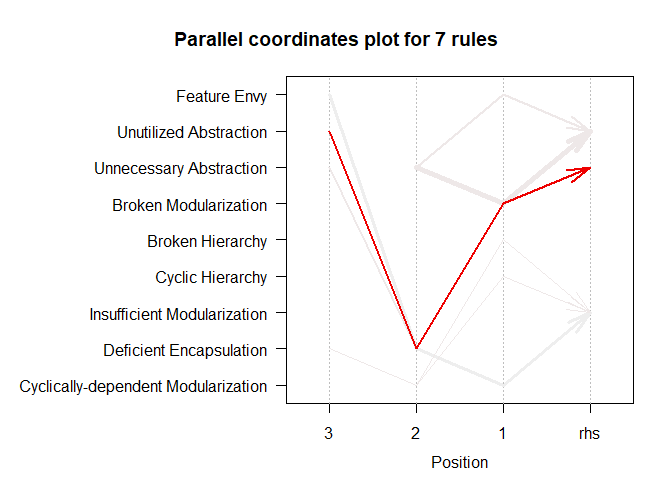
\includegraphics[width=5cm]{img/parallelCoordinateArch.png}
    \caption{Parallel Coordinate Architectural Smells}
    \label{fig:parallelCoordinateArch}
\end{figure}
\begin{figure}[!ht]
    \centering
    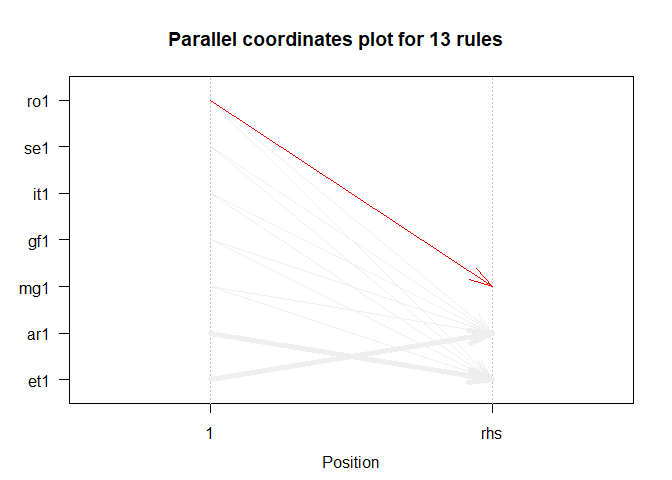
\includegraphics[width=5cm]{img/parallelCoordinateTest.png}
    \caption{Parallel Coordinate Test Smells}
    \label{fig:parallelCoordinateTest}
\end{figure}

For example, Figure \ref{fig:parallelCoordinateTest} shows that when the class has the test smell \textit{'ro1'}, with high probability it will also have the test smell \textit{'mg1'}.
All these plots have been created throw R, the scripts and a report of these results are all reported on GitHub \cite{IEEEhowto:rNotebook}.\par\hfill\par\hfill\par\hfill\par\hfill
